\documentclass[14pt,a4paper]{extarticle}

\usepackage{iftex}
\ifPDFTeX
  \usepackage[T2A]{fontenc}
  \usepackage[utf8]{inputenc}
  \usepackage[english,russian]{babel}
  \IfFileExists{tempora.sty}{\usepackage{tempora}}{}
\else
  \usepackage{fontspec}
  \IfFontExistsTF{Times New Roman}{\setmainfont{Times New Roman}}{%
    \IfFontExistsTF{Liberation Serif}{\setmainfont{Liberation Serif}}{\setmainfont{CMU Serif}}}
  \usepackage[english,russian]{babel}
\fi

\usepackage[left=30mm,right=15mm,top=20mm,bottom=20mm]{geometry}
\usepackage{setspace}
\onehalfspacing
\setlength{\parindent}{1.25cm}
\usepackage{indentfirst}
\usepackage{graphicx}
\usepackage{float}
\usepackage{pdflscape}
\usepackage{needspace}
\usepackage{array}
\usepackage{xltabular}
\usepackage{booktabs}
\usepackage{enumitem}
\setlist{nosep,leftmargin=*,labelindent=\parindent}
\usepackage[labelsep=endash,font=small]{caption}
\usepackage{titlesec}
\titleformat{\section}{\normalfont\large\bfseries}{\thesection}{1em}{}
\titleformat{\subsection}{\normalfont\normalsize\bfseries}{\thesubsection}{1em}{}
\usepackage[hidelinks]{hyperref}

\renewcommand{\arraystretch}{1.15}
\newcolumntype{L}{>{\raggedright\arraybackslash}X}

\newcommand{\teacher}{Тюрин И. Н.}

\newenvironment{usecase}[2]{%
  \par\medskip\noindent\begingroup\small\setstretch{1.1}%
  \begin{tabular}{|>{\bfseries\raggedright\arraybackslash}p{4.2cm}|>{\raggedright\arraybackslash}p{\dimexpr\textwidth-4.2cm-4\tabcolsep-3\arrayrulewidth\relax}|}
  \hline
  \multicolumn{2}{|l|}{\normalsize\textbf{#1. #2}}\\ \hline
}{%
  \end{tabular}
  \endgroup\par\medskip
}
\newcommand{\ucrow}[2]{#1 & #2 \\ \hline}

\begin{document}

\begin{titlepage}
  \centering
  \vspace*{5mm}
  Федеральное государственное автономное образовательное учреждение\\
  высшего образования «Национальный исследовательский университет\\
  ИТМО»\par
  \vspace{4mm}
  \textit{Факультет программной инженерии и компьютерной техники}\\
  \textit{Направление подготовки: 09.03.04 -- Программная инженерия, Системное}\\
  \textit{и прикладное программное обеспечение}\par
  \vspace{18mm}
  Дисциплина: Информационные системы\par
  \vspace{30mm}
  {\large\bfseries Курсовая работа\par}
  \vspace{1mm}
  {\large Информационная система студии сайкл-тренировок\par}
  \vfill
  \begin{flushright}
    Выполнил:\\
    Гришин Артем Евгеньевич\\
    Группа: Р3311\\[3mm]
    Проверил:\\
    \teacher
  \end{flushright}
  \vspace{25mm}
  г. Санкт-Петербург, 2026\par
\end{titlepage}

\tableofcontents
\newpage

\section{Описание предметной области}

\subsection{Студия и места проведения}

Студия сайкл-тренировок --- малое предприятие (индивидуальный предприниматель), которое проводит групповые тренировки на стационарных велотренажёрах (сайклах). Тренировка идёт под музыку: тренер задаёт темп, группа повторяет за ним. Занятие длится фиксированное время, обычно 45--60 минут, и у каждого занятия своя программа и музыкальный плейлист.

У студии одно или несколько мест проведения занятий (филиалов, залов).

Доход студии --- продажа разовых занятий и абонементов.

\subsection{Участники}

\begin{itemize}
  \item \textbf{Клиент} --- человек, который посещает тренировки и оплачивает их. О клиенте известны имя, телефон и/или электронная почта, фотография. Клиент может прийти по приглашению другого клиента.
  \item \textbf{Тренер} --- сотрудник, который ведёт занятия и составляет расписание своих занятий. О тренере известны описание (опыт, специализация), отзывы на него, фотографии и то, работает ли он сейчас в студии. На одном занятии может работать несколько тренеров, у каждого своя роль, например ведущий и ассистент.
  \item \textbf{Администратор} --- сотрудник студии (часто сам владелец). Устанавливает цены, разбирает спорные ситуации с клиентами.
\end{itemize}

\subsection{Занятия}

У \textbf{занятия} есть название, место проведения, дата и время начала, продолжительность в минутах, вместимость, ссылка на плейлист, тренеры с их ролями и статус: запланировано или отменено.

\subsection{Тарифы и абонементы}

\textbf{Тариф} --- позиция прайса студии. У тарифа есть название, описание, цена, признак «в продаже» и вид:
\begin{itemize}
  \item \textbf{разовое занятие} --- одно посещение;
  \item \textbf{пакет} --- заданное число посещений;
  \item \textbf{абонемент на период} --- безлимитные посещения в течение заданного числа дней.
\end{itemize}

\textbf{Абонемент} --- купленный клиентом тариф. У абонемента есть владелец, тариф, дата окончания, остаток занятий (у безлимитного не ограничен) и статус: действует, истёк, использован или возвращён. Разовое занятие тоже оформляется абонементом на одно посещение. Абонемент выдаётся после оплаты либо бесплатно, например в качестве компенсации или награды за приглашённого друга.

\subsection{Оплата}

Клиент оплачивает тариф картой через платёжный сервис, одна оплата --- один тариф. У \textbf{платежа} есть клиент, тариф, сумма, статус (ожидает оплаты, оплачен, отменён, возвращён) и дата оплаты. При возврате фиксируются сумма возврата (полная или частичная) и его дата.

Клиент может сохранить карту для следующих оплат. У \textbf{сохранённой карты} есть владелец, последние четыре цифры номера, платёжная система, срок действия и признак, действует ли она. Платёж может быть проведён сохранённой картой.

\subsection{Запись на занятие}

\textbf{Запись} связывает клиента, занятие и абонемент, с которого списано посещение. Статус записи: записан, пришёл, не пришёл, отменена; для отменённой записи известно время отмены. При ранней отмене занятие возвращается на абонемент, при поздней отмене и неявке --- сгорает.

\subsection{Отзывы}

Клиент оставляет \textbf{отзыв} о тренере: оценку от 1 до 5 и текст. От одного клиента о тренере может быть только один отзыв.

\subsection{Документы}

Студия публикует \textbf{документы}: правила студии, политику обработки персональных данных и публичную оферту. У документа есть название, файл, вид, номер редакции и признак, действует ли он. При регистрации клиент соглашается с документами; дата согласия сохраняется.

\section{Назначение информационной системы}

Сейчас студия использует CRM-систему, в которой есть только приём оплаты. Записи, расписание и абонементы ведутся вручную в переписке с клиентами, поэтому и клиенты, и сотрудники испытывают большие неудобства:
\begin{itemize}
  \item клиент не видит актуальное расписание и свободные места и записывается через администратора;
  \item остаток занятий по абонементу считается через сторонние сервисы, что вызывает неудобство;
  \item бывают двойные записи и переполненные занятия;
  \item нет данных о посещаемости, загрузке занятий и популярности тренеров.
\end{itemize}

\textbf{Цель} информационной системы --- автоматизировать запись на тренировки, продажу и учёт абонементов, чтобы клиенты записывались сами, а сотрудники не вели учёт вручную.

\textbf{Задачи} системы:
\begin{enumerate}
  \item Публикация расписания, карточек тренеров, мест проведения и тарифов.
  \item Запись на занятия и отмена записи.
  \item Онлайн-продажа тарифов и учёт абонементов.
  \item Учёт посещаемости.
  \item Сбор отзывов о тренерах.
  \item Реферальная программа.
  \item Ведение статистики: посещаемость, загрузка занятий, рейтинг тренеров, выручка.
\end{enumerate}

\section{Требования к информационной системе}

\subsection{Функциональные требования}

\begingroup\small
\begin{xltabular}{\textwidth}{|p{1.4cm}|L|}
  \hline
  \textbf{Код} & \textbf{Требование} \\ \hline
  \endhead
  \multicolumn{2}{|l|}{\textit{Регистрация и вход}} \\ \hline
  ФТ-1 & Регистрация по телефону или электронной почте с паролем. \\ \hline
  ФТ-2 & Регистрация через VK ID. \\ \hline
  ФТ-3 & Регистрация через Google. \\ \hline
  ФТ-4 & Регистрация возможна только после отметки согласия с правилами студии, политикой обработки ПДн и офертой. \\ \hline
  ФТ-5 & Указание кода приглашения при регистрации. \\ \hline
  ФТ-6 & Вход по телефону или почте и паролю. \\ \hline
  ФТ-7 & Вход через VK ID. \\ \hline
  ФТ-8 & Вход через Google. \\ \hline
  ФТ-9 & Восстановление пароля. \\ \hline
  ФТ-10 & Редактирование профиля: имя, телефон, почта, фотография. \\ \hline
  \multicolumn{2}{|l|}{\textit{Информация о студии}} \\ \hline
  ФТ-11 & Просмотр расписания занятий с числом свободных мест. \\ \hline
  ФТ-12 & Фильтрация расписания по месту проведения, тренеру и дате. \\ \hline
  ФТ-13 & Просмотр карточки тренера: описание, фотографии, средняя оценка, отзывы. \\ \hline
  ФТ-14 & Просмотр тарифов в продаже. \\ \hline
  ФТ-15 & Просмотр мест проведения. \\ \hline
  \multicolumn{2}{|l|}{\textit{Запись на занятия}} \\ \hline
  ФТ-16 & Запись на занятие со списанием одного занятия с действующего абонемента. \\ \hline
  ФТ-17 & Запрет записи при отсутствии свободных мест. \\ \hline
  ФТ-18 & Запрет повторной записи на одно занятие. \\ \hline
  ФТ-19 & Отмена записи клиентом. \\ \hline
  ФТ-20 & Возврат занятия на абонемент при отмене не позднее установленного срока. \\ \hline
  ФТ-21 & Просмотр клиентом своих предстоящих и прошедших записей. \\ \hline
  \multicolumn{2}{|l|}{\textit{Тарифы, абонементы, оплата}} \\ \hline
  ФТ-22 & Покупка тарифа с онлайн-оплатой картой. \\ \hline
  ФТ-23 & Создание абонемента после успешной оплаты. \\ \hline
  ФТ-24 & Просмотр клиентом своих абонементов: остаток занятий, дата окончания, статус. \\ \hline
  ФТ-25 & Просмотр клиентом истории платежей. \\ \hline
  ФТ-26 & Перевод абонемента в статус «истёк» по окончании срока. \\ \hline
  ФТ-27 & Перевод абонемента в статус «использован», когда закончились занятия. \\ \hline
  ФТ-28 & Сохранение карты при оплате с согласия клиента. \\ \hline
  ФТ-29 & Оплата тарифа сохранённой картой. \\ \hline
  ФТ-30 & Просмотр сохранённых карт в личном кабинете. \\ \hline
  ФТ-31 & Удаление сохранённой карты. \\ \hline
  \multicolumn{2}{|l|}{\textit{Реферальная программа и отзывы}} \\ \hline
  ФТ-32 & Отображение личного кода приглашения в профиле клиента. \\ \hline
  ФТ-33 & Выдача пригласившему бесплатного разового занятия после первой оплаты приглашённого. \\ \hline
  ФТ-34 & Отзыв о тренере (оценка 1--5 и текст) от клиента, посещавшего его занятие. \\ \hline
  ФТ-35 & Изменение клиентом своего отзыва. \\ \hline
  \multicolumn{2}{|l|}{\textit{Функции тренера}} \\ \hline
  ФТ-36 & Создание занятия: название, место, время, длительность, вместимость, плейлист, тренеры и их роли. \\ \hline
  ФТ-37 & Изменение своего занятия. \\ \hline
  ФТ-38 & Отмена своего занятия с возвратом занятий всем записавшимся. \\ \hline
  ФТ-39 & Просмотр списка записавшихся на своё занятие. \\ \hline
  ФТ-40 & Отметка посещения: «пришёл» / «не пришёл». \\ \hline
  ФТ-41 & Редактирование описания в своей карточке. \\ \hline
  ФТ-42 & Загрузка фотографий в карточку и выбор их порядка. \\ \hline
  \multicolumn{2}{|l|}{\textit{Функции администратора}} \\ \hline
  ФТ-43 & Создание, изменение и снятие с продажи тарифов. \\ \hline
  ФТ-44 & Создание, изменение и закрытие мест проведения. \\ \hline
  ФТ-45 & Назначение пользователя тренером и отключение тренера. \\ \hline
  ФТ-46 & Загрузка документов и их новых редакций. \\ \hline
  ФТ-47 & Полный или частичный возврат платежа. \\ \hline
  ФТ-48 & Выдача клиенту абонемента без оплаты. \\ \hline
  ФТ-49 & Просмотр статистики посещаемости и загрузки занятий. \\ \hline
  ФТ-50 & Просмотр рейтинга тренеров. \\ \hline
  ФТ-51 & Просмотр выручки по тарифам и периодам. \\ \hline
\end{xltabular}
\endgroup

\subsection{Нефункциональные требования}

\begingroup\small
\begin{xltabular}{\textwidth}{|p{1.6cm}|L|}
  \hline
  \textbf{Код} & \textbf{Требование} \\ \hline
  \endhead
  НФТ-1 & Запись на занятие и списание занятия с абонемента выполняются в одной транзакции. \\ \hline
  НФТ-2 & При одновременной записи на последнее место вместимость занятия не превышается. \\ \hline
  НФТ-3 & Повторное уведомление платёжного сервиса об одной оплате не создаёт второй абонемент. \\ \hline
  НФТ-4 & Корректность данных проверяется на каждом уровне системы. Ограничения целостности в СУБД действуют независимо от проверок в приложении. \\ \hline
  НФТ-5 & Пароли хранятся в виде хеша (bcrypt). \\ \hline
  НФТ-6 & Обмен данными с сервером по HTTPS (TLS 1.2 и выше); браузеру передаётся заголовок HSTS. \\ \hline
  НФТ-7 & Клиент имеет доступ только к своим записям, абонементам и платежам. \\ \hline
  НФТ-8 & Функции тренера и администратора доступны только пользователям с этими ролями. \\ \hline
  НФТ-9 & Номер карты и CVC система не получает и не хранит; для повторной оплаты хранится токен платёжного сервиса. \\ \hline
  НФТ-10 & Персональные данные хранятся на серверах в РФ (152-ФЗ). \\ \hline
  НФТ-11 & Чеки по оплатам формируются онлайн-кассой платёжного сервиса (54-ФЗ). \\ \hline
  НФТ-12 & Журнал изменений базы данных архивируется непрерывно; при сбое теряется не более 15 минут данных. \\ \hline
  НФТ-13 & Резервные копии хранятся вне основного сервера, в хранилище на территории РФ. \\ \hline
  НФТ-14 & 95\,\% типовых запросов выполняются не более чем за 1 с при 100 одновременных пользователях. \\ \hline
  НФТ-15 & Сервер размещается у хостинг-провайдера с защитой от DDoS-атак сетевого уровня. \\ \hline
  НФТ-16 & Число запросов с одного IP-адреса ограничено; при превышении сервер отвечает кодом 429. \\ \hline
  НФТ-17 & Сервер закрывает соединения, по которым запрос не передан за установленное время. \\ \hline
  НФТ-18 & После 5 неудачных попыток входа подряд вход возможен только после прохождения капчи. \\ \hline
  НФТ-19 & Число одновременных соединений с базой данных ограничено пулом соединений. \\ \hline
  НФТ-20 & Расписание, тарифы и карточки тренеров отдаются из кэша, который сбрасывается при каждом их изменении, записи и отмене записи. \\ \hline
  НФТ-21 & Загружаемые фотографии ограничены по размеру и проверяются на формат изображения. \\ \hline
  НФТ-22 & Каждый запрос к внешним сервисам ограничен таймаутом. \\ \hline
  НФТ-23 & Повтор неудачного запроса к платёжному сервису выполняется с экспоненциально растущей паузой со случайной добавкой. \\ \hline
  НФТ-24 & Повторный запрос к платёжному сервису отправляется с тем же ключом идемпотентности и не создаёт второй платёж. \\ \hline
  НФТ-25 & Повторное нажатие «Купить» не создаёт второй платёж. \\ \hline
  НФТ-26 & Уведомление об оплате принимается только после проверки статуса платежа в платёжном сервисе. \\ \hline
  НФТ-27 & Статус платежей, ожидающих оплаты, периодически сверяется с платёжным сервисом. \\ \hline
  НФТ-28 & При недоступности платёжного сервиса остальные функции сайта продолжают работать. \\ \hline
  НФТ-29 & Время хранится с часовым поясом и отображается в часовом поясе места проведения. \\ \hline
  НФТ-30 & Доступность сайта проверяется автоматически; при недоступности администратор системы получает уведомление. \\ \hline
  НФТ-31 & При ошибках приёма оплаты администратор системы получает уведомление. \\ \hline
  НФТ-32 & В журналы не записываются пароли, токены способов оплаты и ключи доступа. \\ \hline
  НФТ-33 & Ключи доступа к платёжному сервису и сервисам входа хранятся вне исходного кода. \\ \hline
  НФТ-34 & При перезапуске сервер завершает обработку текущих запросов. \\ \hline
  НФТ-35 & Идентификатор сессии передаётся в cookie с флагами HttpOnly, Secure и SameSite. \\ \hline
  НФТ-36 & Сессии пользователей сохраняются при перезапуске сервера. \\ \hline
  НФТ-37 & Интерфейс на русском языке, адаптирован под телефон и компьютер. \\ \hline
  НФТ-38 & СУБД PostgreSQL, серверная часть на Java (Spring Boot), клиентская часть на Angular. \\ \hline
\end{xltabular}
\endgroup

\section{Модели основных прецедентов}

\subsection{Актёры}

\begin{itemize}
  \item \textbf{Гость} --- посетитель сайта без учётной записи.
  \item \textbf{Клиент} --- зарегистрированный пользователь; может всё, что гость.
  \item \textbf{Тренер} --- ведёт свои занятия и карточку.
  \item \textbf{Администратор} --- ведёт тарифы, места, тренеров, документы, возвраты.
  \item \textbf{VK ID / Google} --- внешние сервисы входа.
  \item \textbf{Платёжный сервис} --- сервис, который ведёт приём оплат и возвраты.
\end{itemize}
\subsection{Диаграмма прецедентов}

\begin{figure}[H]
  \centering
  \IfFileExists{diagrams/use-case.png}{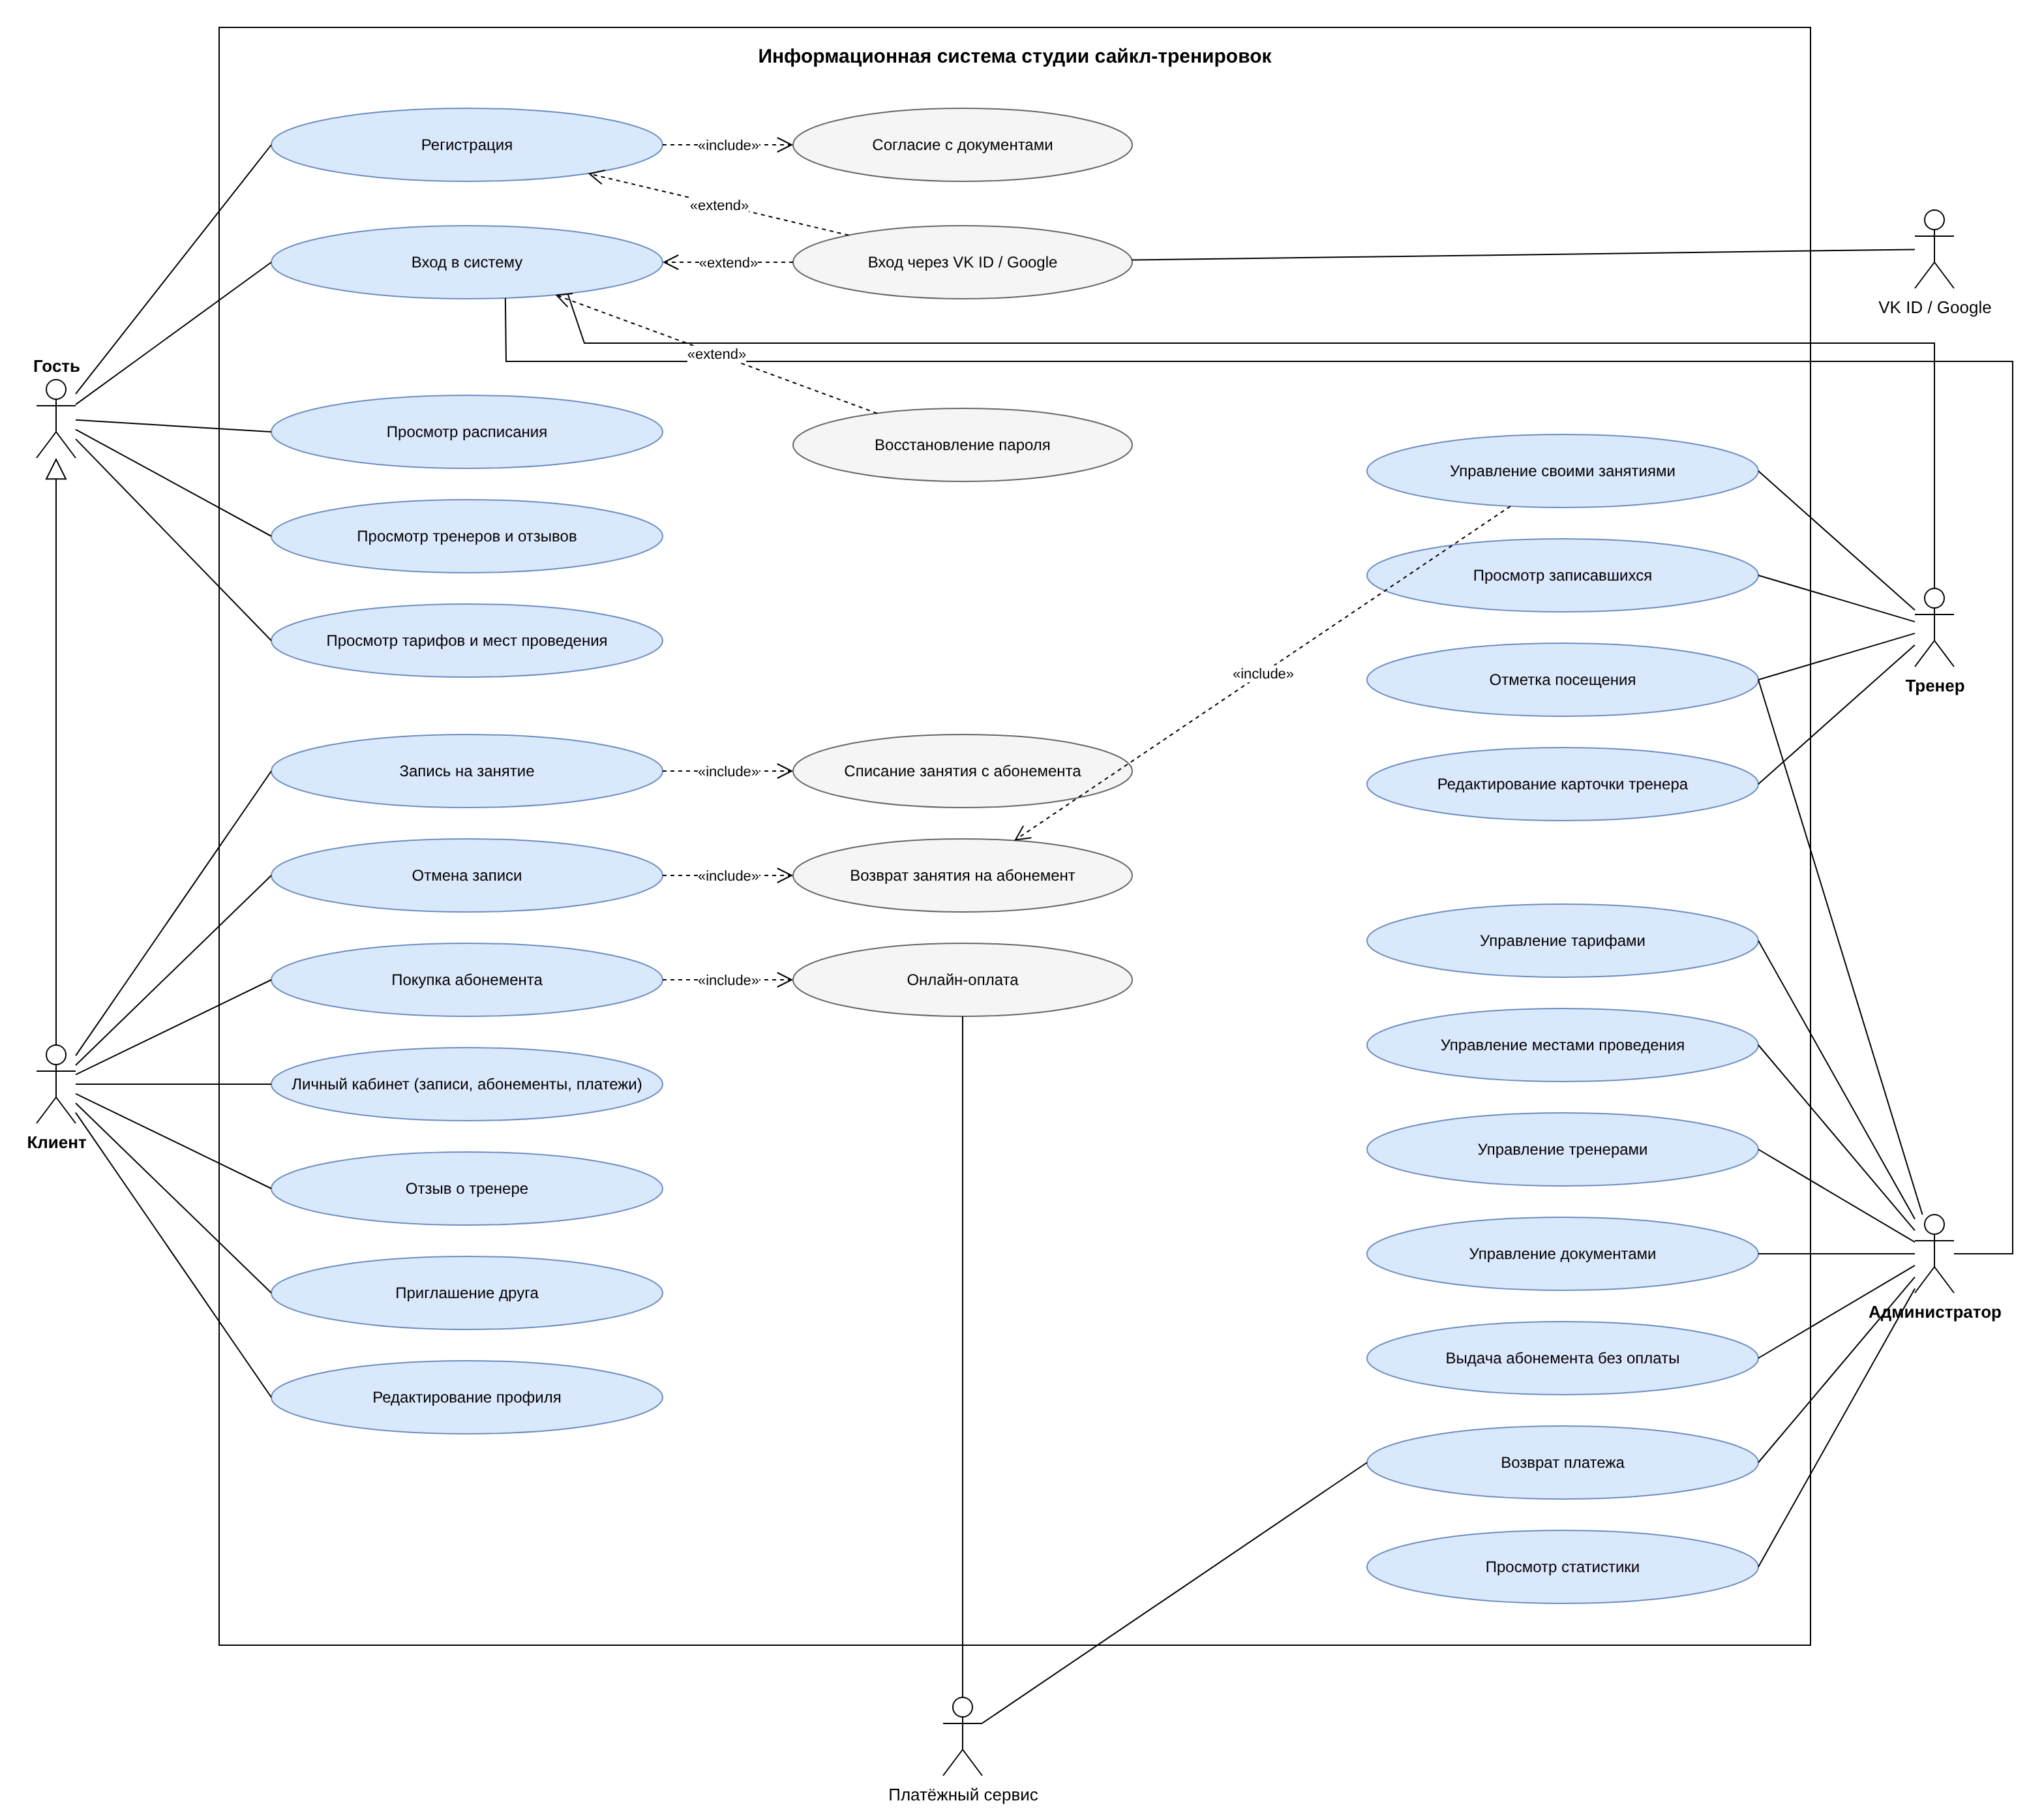
\includegraphics[width=\textwidth]{diagrams/use-case.png}}{\includegraphics[width=\textwidth]{use-case.png}}
  \caption{Диаграмма прецедентов}
  \label{fig:usecase}
\end{figure}

\newpage
\subsection{Описание прецедентов}

\begin{usecase}{UC-1}{Регистрация}
\ucrow{Актёры}{Гость}
\ucrow{Основной поток}{%
1. Гость открывает форму регистрации.\newline
2. Вводит имя, телефон или почту, пароль и, если есть, код приглашения.\newline
3. Отмечает галочки согласия с правилами студии, политикой обработки ПДн и офертой (рядом ссылки на документы).\newline
4. Нажимает «Зарегистрироваться».\newline
5. Система создаёт учётную запись с личным кодом приглашения, сохраняет согласия и выполняет вход.}
\ucrow{Альтернативные потоки}{%
2а. Гость нажимает «Через VK ID» или «Через Google»: имя и почта берутся из аккаунта, пароль не нужен.\newline
3а. Не все галочки отмечены: кнопка регистрации неактивна.\newline
4а. Телефон или почта уже заняты: система предлагает войти.\newline
4б. Код приглашения не найден: система сообщает об ошибке.}
\ucrow{Результат}{Создана учётная запись клиента.}
\end{usecase}

\begin{usecase}{UC-2}{Вход в систему}
\ucrow{Актёры}{Гость, Тренер, Администратор, VK ID / Google}
\ucrow{Основной поток}{%
1. Пользователь вводит телефон или почту и пароль.\newline
2. Система проверяет пароль и открывает личный кабинет его роли.}
\ucrow{Альтернативные потоки}{%
1а. Пользователь нажимает «Через VK ID» или «Через Google» и подтверждает вход во внешнем сервисе.\newline
2а. Неверный пароль: система сообщает об ошибке.\newline
2б. Пользователь нажимает «Забыли пароль?»: на почту или телефон приходит ссылка для смены пароля.}
\ucrow{Результат}{Пользователь вошёл в систему.}
\end{usecase}

\begin{usecase}{UC-3}{Запись на занятие}
\ucrow{Актёры}{Клиент}
\ucrow{Предусловия}{Клиент вошёл в систему.}
\ucrow{Основной поток}{%
1. Клиент выбирает занятие в расписании и нажимает «Записаться».\newline
2. Если у клиента несколько действующих абонементов, он выбирает, с какого списать занятие.\newline
3. Система проверяет, что есть свободные места и клиент ещё не записан.\newline
4. Система списывает одно занятие с абонемента и создаёт запись.}
\ucrow{Альтернативные потоки}{%
2а. Действующего абонемента нет: система предлагает купить тариф (UC-5), затем возвращается к шагу 3.\newline
3а. Мест нет: кнопка «Записаться» неактивна.\newline
3б. Клиент уже записан: вместо кнопки показано «Вы записаны».}
\ucrow{Результат}{Клиент записан, остаток абонемента уменьшен на одно занятие.}
\end{usecase}

\begin{usecase}{UC-4}{Отмена записи}
\ucrow{Актёры}{Клиент}
\ucrow{Предусловия}{У клиента есть запись на ещё не начавшееся занятие.}
\ucrow{Основной поток}{%
1. Клиент нажимает «Отменить» у записи в личном кабинете.\newline
2. Система предупреждает, вернётся ли занятие на абонемент, клиент подтверждает.\newline
3. Система отменяет запись и при ранней отмене возвращает занятие на абонемент.}
\ucrow{Результат}{Запись отменена, место освобождено.}
\end{usecase}

\begin{usecase}{UC-5}{Покупка абонемента}
\ucrow{Актёры}{Клиент, Платёжный сервис}
\ucrow{Предусловия}{Клиент вошёл в систему.}
\ucrow{Основной поток}{%
1. Клиент выбирает тариф и нажимает «Купить».\newline
2. Система создаёт платёж и открывает страницу оплаты платёжного сервиса.\newline
3. Клиент оплачивает картой.\newline
4. Платёжный сервис сообщает об успешной оплате.\newline
5. Система создаёт абонемент.\newline
6. Если клиент пришёл по приглашению и это его первая оплата, пригласивший получает бесплатное разовое занятие.}
\ucrow{Альтернативные потоки}{%
3а. Оплата не прошла или клиент закрыл страницу: платёж отменяется, абонемент не создаётся.}
\ucrow{Результат}{У клиента новый абонемент.}
\end{usecase}

\begin{usecase}{UC-6}{Отзыв о тренере}
\ucrow{Актёры}{Клиент}
\ucrow{Предусловия}{Клиент посещал занятие этого тренера.}
\ucrow{Основной поток}{%
1. Клиент открывает карточку тренера и нажимает «Оставить отзыв».\newline
2. Ставит оценку от 1 до 5, пишет текст и сохраняет.}
\ucrow{Альтернативные потоки}{%
1а. Отзыв уже есть: вместо кнопки «Оставить отзыв» --- «Изменить отзыв».}
\ucrow{Результат}{Отзыв виден на карточке тренера.}
\end{usecase}

\begin{usecase}{UC-7}{Управление своими занятиями}
\ucrow{Актёры}{Тренер}
\ucrow{Основной поток}{%
1. Тренер нажимает «Добавить занятие».\newline
2. Указывает название, место, дату и время, длительность, вместимость, плейлист, других тренеров и их роли.\newline
3. Система проверяет, что вместимость не больше вместимости места, и публикует занятие в расписании.}
\ucrow{Альтернативные потоки}{%
1а. Изменение: тренер меняет данные занятия; вместимость нельзя сделать меньше числа записанных.\newline
1б. Отмена: система отменяет занятие и все записи на него и возвращает занятия на абонементы.}
\ucrow{Результат}{Расписание обновлено.}
\end{usecase}

\begin{usecase}{UC-8}{Отметка посещения}
\ucrow{Актёры}{Тренер, Администратор}
\ucrow{Основной поток}{%
1. Тренер открывает своё занятие и видит список записавшихся.\newline
2. Отмечает у каждого «пришёл» или «не пришёл».}
\ucrow{Результат}{Посещение учтено.}
\end{usecase}

\begin{usecase}{UC-9}{Возврат платежа}
\ucrow{Актёры}{Администратор, Платёжный сервис}
\ucrow{Основной поток}{%
1. Администратор находит платёж клиента и видит, сколько занятий по абонементу использовано.\newline
2. Вводит сумму возврата: полную или частичную.\newline
3. Система отправляет возврат в платёжный сервис.\newline
4. После подтверждения платёж и абонемент получают статус «возвращён».}
\ucrow{Альтернативные потоки}{%
2а. Сумма больше суммы платежа: система не принимает её.\newline
3а. Платёжный сервис отклонил возврат: статусы не меняются.}
\ucrow{Результат}{Деньги возвращены, абонемент не действует.}
\end{usecase}

\begin{usecase}{UC-10}{Выдача абонемента без оплаты}
\ucrow{Актёры}{Администратор}
\ucrow{Основной поток}{%
1. Администратор находит клиента по имени, телефону или почте.\newline
2. Выбирает тариф и нажимает «Выдать».}
\ucrow{Результат}{У клиента новый абонемент, не связанный с платежом.}
\end{usecase}

\sloppy
\section{Архитектура и технологии}

\subsection{Общая схема}

Система строится по клиент-серверной архитектуре из трёх частей:
\begin{itemize}
  \item \textbf{клиент} --- одностраничное веб-приложение на Angular, работает в браузере;
  \item \textbf{сервер приложений} --- Spring Boot (Java 17), отдаёт данные клиенту через REST API в формате JSON;
  \item \textbf{база данных} --- PostgreSQL.
\end{itemize}

Сервер также обращается к внешним сервисам: ЮKassa (оплата, возвраты, сохранённые карты), VK ID и Google (вход).

\subsection{Клиентская часть}

Angular построен по схеме MVVM: шаблон компонента (представление) связан с полями класса компонента (модель представления) привязкой данных, а обращения к серверу вынесены в сервисы. Каждая страница сайта --- отдельный компонент: расписание, карточка тренера, тарифы, личный кабинет, кабинеты тренера и администратора. Доступ к страницам кабинетов закрыт по роли пользователя, но окончательная проверка прав выполняется на сервере.

\subsection{Серверная часть}

Сервер написан на Spring Boot (Spring MVC) и разделён на три слоя:
\begin{itemize}
  \item \textbf{контроллеры} принимают HTTP-запросы и возвращают JSON;
  \item \textbf{сервисы} содержат бизнес-логику и задают границы транзакций: например, запись на занятие и списание занятия с абонемента выполняются в одной транзакции;
  \item \textbf{репозитории} (Spring Data JPA) работают с базой данных.
\end{itemize}

Вход и роли реализуются через Spring Security, сессии хранятся в базе данных (Spring Session JDBC), поэтому переживают перезапуск сервера. Схема базы данных создаётся и меняется миграциями Flyway.

\subsection{Модульный монолит}

Сервер собирается в одно приложение, но код разделён на модули по предметным областям:
\begin{itemize}
  \item \textbf{пользователи и вход} --- регистрация, профиль, согласия, вход через VK ID и Google, реферальные коды;
  \item \textbf{расписание и запись} --- места проведения, занятия, тренеры, записи, отметка посещения;
  \item \textbf{тарифы и оплата} --- тарифы, абонементы, платежи, возвраты, сохранённые карты;
  \item \textbf{отзывы};
  \item \textbf{документы};
  \item \textbf{статистика} --- только чтение через представления (VIEW) базы данных.
\end{itemize}

Модуль обращается к другому модулю только через его сервис, а не напрямую к его таблицам. Микросервисы не используются: нагрузка одной студии не требует раздельного масштабирования частей системы.

\subsection{Подключение внешних сервисов}

\textbf{ЮKassa.} Сервер работает с REST API ЮKassa версии 3 (\texttt{https://api.yookassa.ru/v3/}), данные передаются в JSON. Каждый запрос подписывается по схеме HTTP Basic: логин --- идентификатор магазина, пароль --- секретный ключ из личного кабинета ЮKassa. К каждому POST-запросу добавляется заголовок \texttt{Idempotence-Key}: повтор запроса с тем же ключом не создаёт второй платёж. Официального SDK для Java у ЮKassa нет, поэтому клиент пишется на Spring \texttt{RestClient}.

Оплата тарифа:
\begin{enumerate}
  \item Сервер создаёт платёж запросом \texttt{POST /payments}: сумма, описание, данные для чека, адрес возврата на сайт и, если клиент отметил «Запомнить карту», признак сохранения способа оплаты.
  \item ЮKassa возвращает идентификатор платежа и ссылку на страницу оплаты, клиент переходит по ней и вводит данные карты.
  \item О результате ЮKassa сообщает HTTP-уведомлением (\texttt{payment.succeeded} или \texttt{payment.canceled}) на адрес сервера, указанный в личном кабинете. Сервер проверяет статус запросом \texttt{GET /payments/\{id\}} и создаёт абонемент.
  \item Если карта сохранена, в ответе приходят идентификатор способа оплаты, последние четыре цифры и тип карты. Следующая оплата этой картой --- запрос \texttt{POST /payments} с идентификатором способа оплаты, без перехода на страницу оплаты.
\end{enumerate}

Возврат --- запрос \texttt{POST /refunds} с идентификатором платежа и суммой, о завершении приходит уведомление \texttt{refund.succeeded}.

\textbf{Google.} Вход работает по протоколу OpenID Connect. В Google Cloud Console создаётся OAuth-клиент: идентификатор, секрет и адрес возврата на сайт. Вход реализуется модулем OAuth2 Login из Spring Security, в котором Google --- встроенный провайдер, поэтому достаточно указать идентификатор и секрет клиента. Пользователь перенаправляется на страницу входа Google, возвращается на сайт с кодом, сервер обменивает код на токены и берёт из ID-токена идентификатор пользователя (\texttt{sub}, сохраняется в \texttt{google\_id}), почту и имя.

\textbf{VK ID.} Вход работает по протоколу OAuth 2.1 с PKCE. Приложение регистрируется в кабинете VK ID для бизнеса и получает идентификатор приложения.
\begin{enumerate}
  \item Сайт перенаправляет пользователя на \texttt{https://id.vk.ru/authorize} с идентификатором приложения, адресом возврата, строкой \texttt{state} и \texttt{code\_challenge} --- хешем SHA-256 от случайной строки \texttt{code\_verifier}.
  \item После подтверждения VK возвращает на сайт \texttt{code}, \texttt{state} и \texttt{device\_id}.
  \item Сервер обменивает код на токен запросом \texttt{POST https://id.vk.ru/oauth2/auth} с \texttt{code}, \texttt{code\_verifier}, \texttt{device\_id} и \texttt{state} и получает \texttt{access\_token} и идентификатор пользователя VK (сохраняется в \texttt{vk\_id}).
  \item По \texttt{access\_token} сервер запрашивает имя и почту пользователя.
\end{enumerate}
VK ID нет среди встроенных провайдеров Spring Security, а обмен кода требует нестандартного параметра \texttt{device\_id}, поэтому этот обмен реализуется отдельным обработчиком.

\section{ER-модель}

ER-модель построена в нотации Мартина (рис.~\ref{fig:er}) и содержит 14 сущностей: Пользователь, Администратор, Тренер, Фото тренера, Отзыв, Место проведения, Занятие, Запись, Тариф, Абонемент, Платёж, Сохранённая карта, Юридический документ, Согласие.

\begin{figure}[H]
  \centering
  \IfFileExists{diagrams/er-model.png}{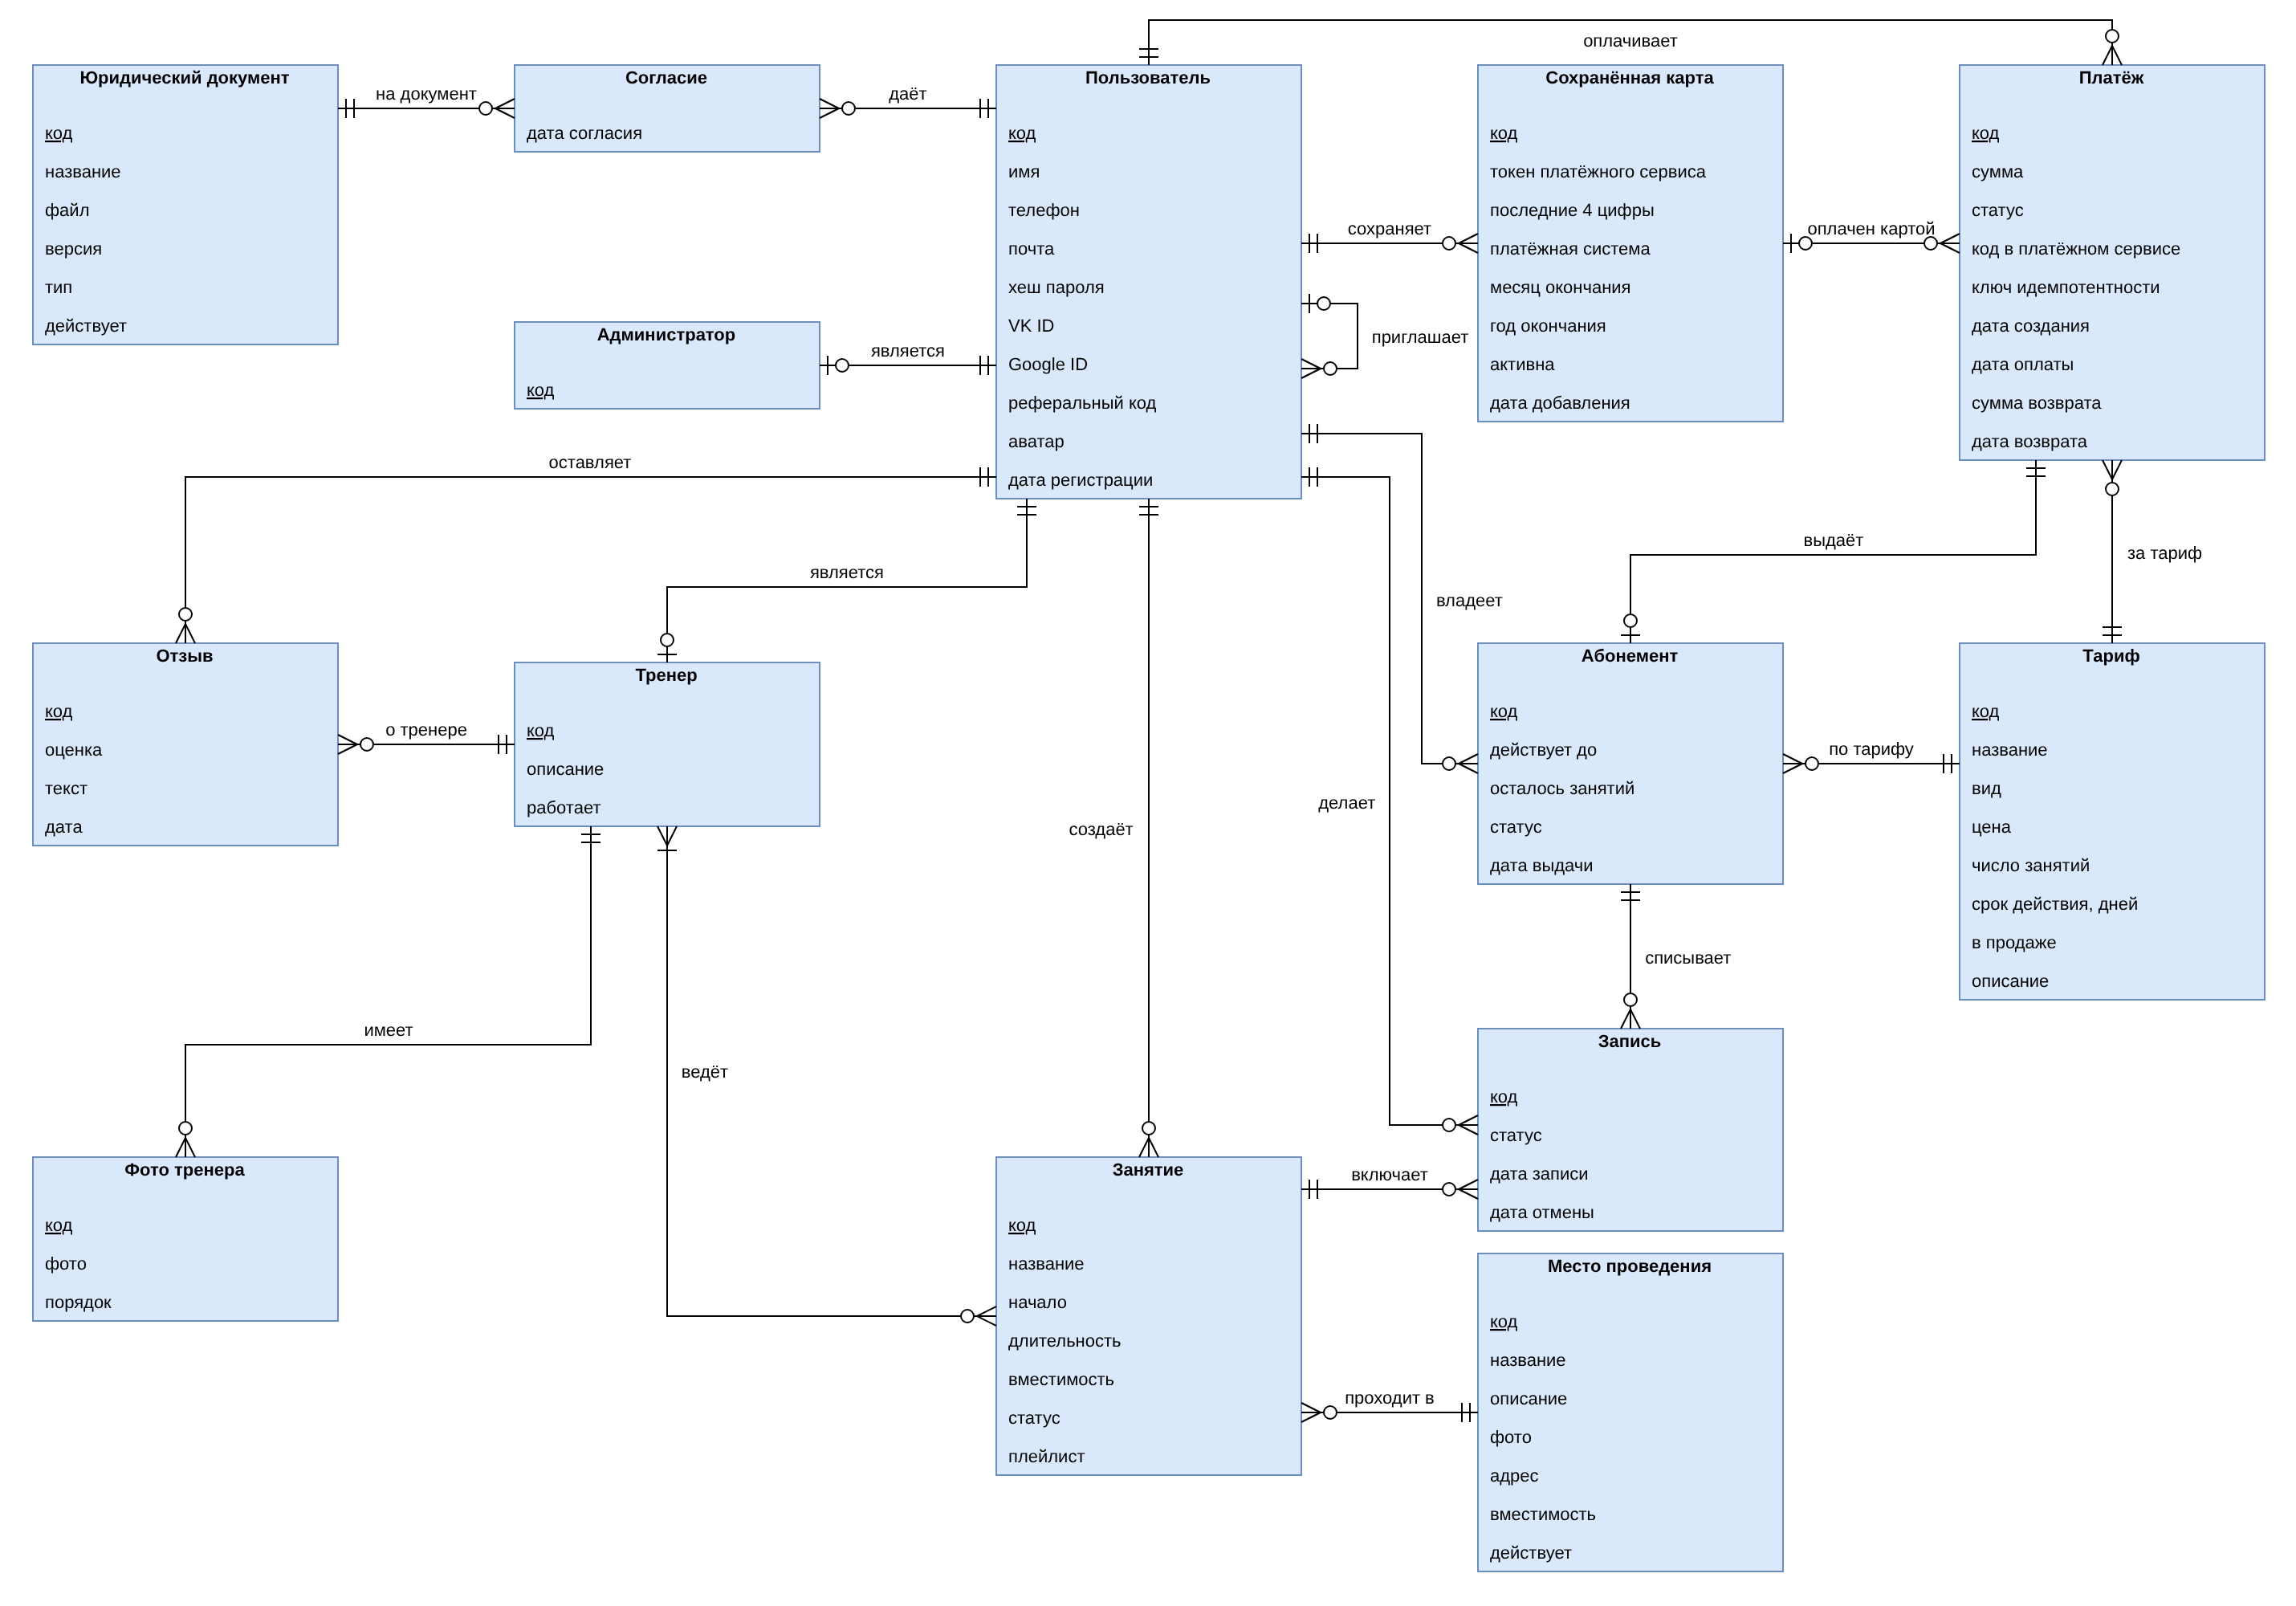
\includegraphics[width=\textwidth]{diagrams/er-model.png}}{\includegraphics[width=\textwidth]{er-model.png}}
  \caption{ER-модель}
  \label{fig:er}
\end{figure}

Связи модели:
\begin{itemize}
  \item \textbf{Тренер --- Занятие} («ведёт») --- связь «многие-ко-многим»: тренер ведёт много занятий, на одном занятии может работать несколько тренеров.
  \item \textbf{Пользователь --- Занятие} тоже по смыслу «многие-ко-многим»: клиент ходит на много занятий, на занятие записано много клиентов. Эта связь разрешена через сущность \textbf{Запись}, потому что у неё есть свои атрибуты (статус, дата записи, дата отмены) и своя связь с Абонементом, с которого списано посещение.
  \item \textbf{Пользователь --- Юридический документ} аналогично разрешена через сущность \textbf{Согласие} с атрибутом «дата согласия».
  \item \textbf{Тренер} и \textbf{Администратор} --- роли Пользователя (связь «один к нулю или одному»): у тренера есть свои атрибуты (описание, признак «работает»), у администратора --- только принадлежность к роли.
  \item \textbf{Пользователь --- Пользователь} («приглашает») --- рекурсивная связь «один-ко-многим»: один клиент может пригласить многих.
  \item \textbf{Платёж --- Абонемент} («выдаёт») --- «один к нулю или одному»: абонемент, выданный бесплатно, не связан с платежом.
  \item \textbf{Сохранённая карта --- Платёж} («оплачен картой») --- необязательная связь: платёж может быть проведён без сохранённой карты.
  \item Остальные связи «один-ко-многим»: Пользователь оставляет Отзывы о Тренере, Тренер имеет Фото, Занятие проходит в Месте проведения и создаётся Пользователем, Абонемент оформлен по Тарифу, Платёж --- за Тариф.
\end{itemize}

\section{Даталогическая модель}

По сравнению с ER-моделью в даталогической модели добавлена одна таблица --- \texttt{activity\_trainer}. Связь «многие-ко-многим» «ведёт» между Тренером и Занятием в реляционной базе данных реализуется через отдельную таблицу с составным первичным ключом (\texttt{activity\_id}, \texttt{trainer\_id}). В этой же таблице хранится роль тренера на занятии (\texttt{role}).

\begin{landscape}
\begin{figure}[p]
  \centering
  \IfFileExists{diagrams/datalogical-model.png}{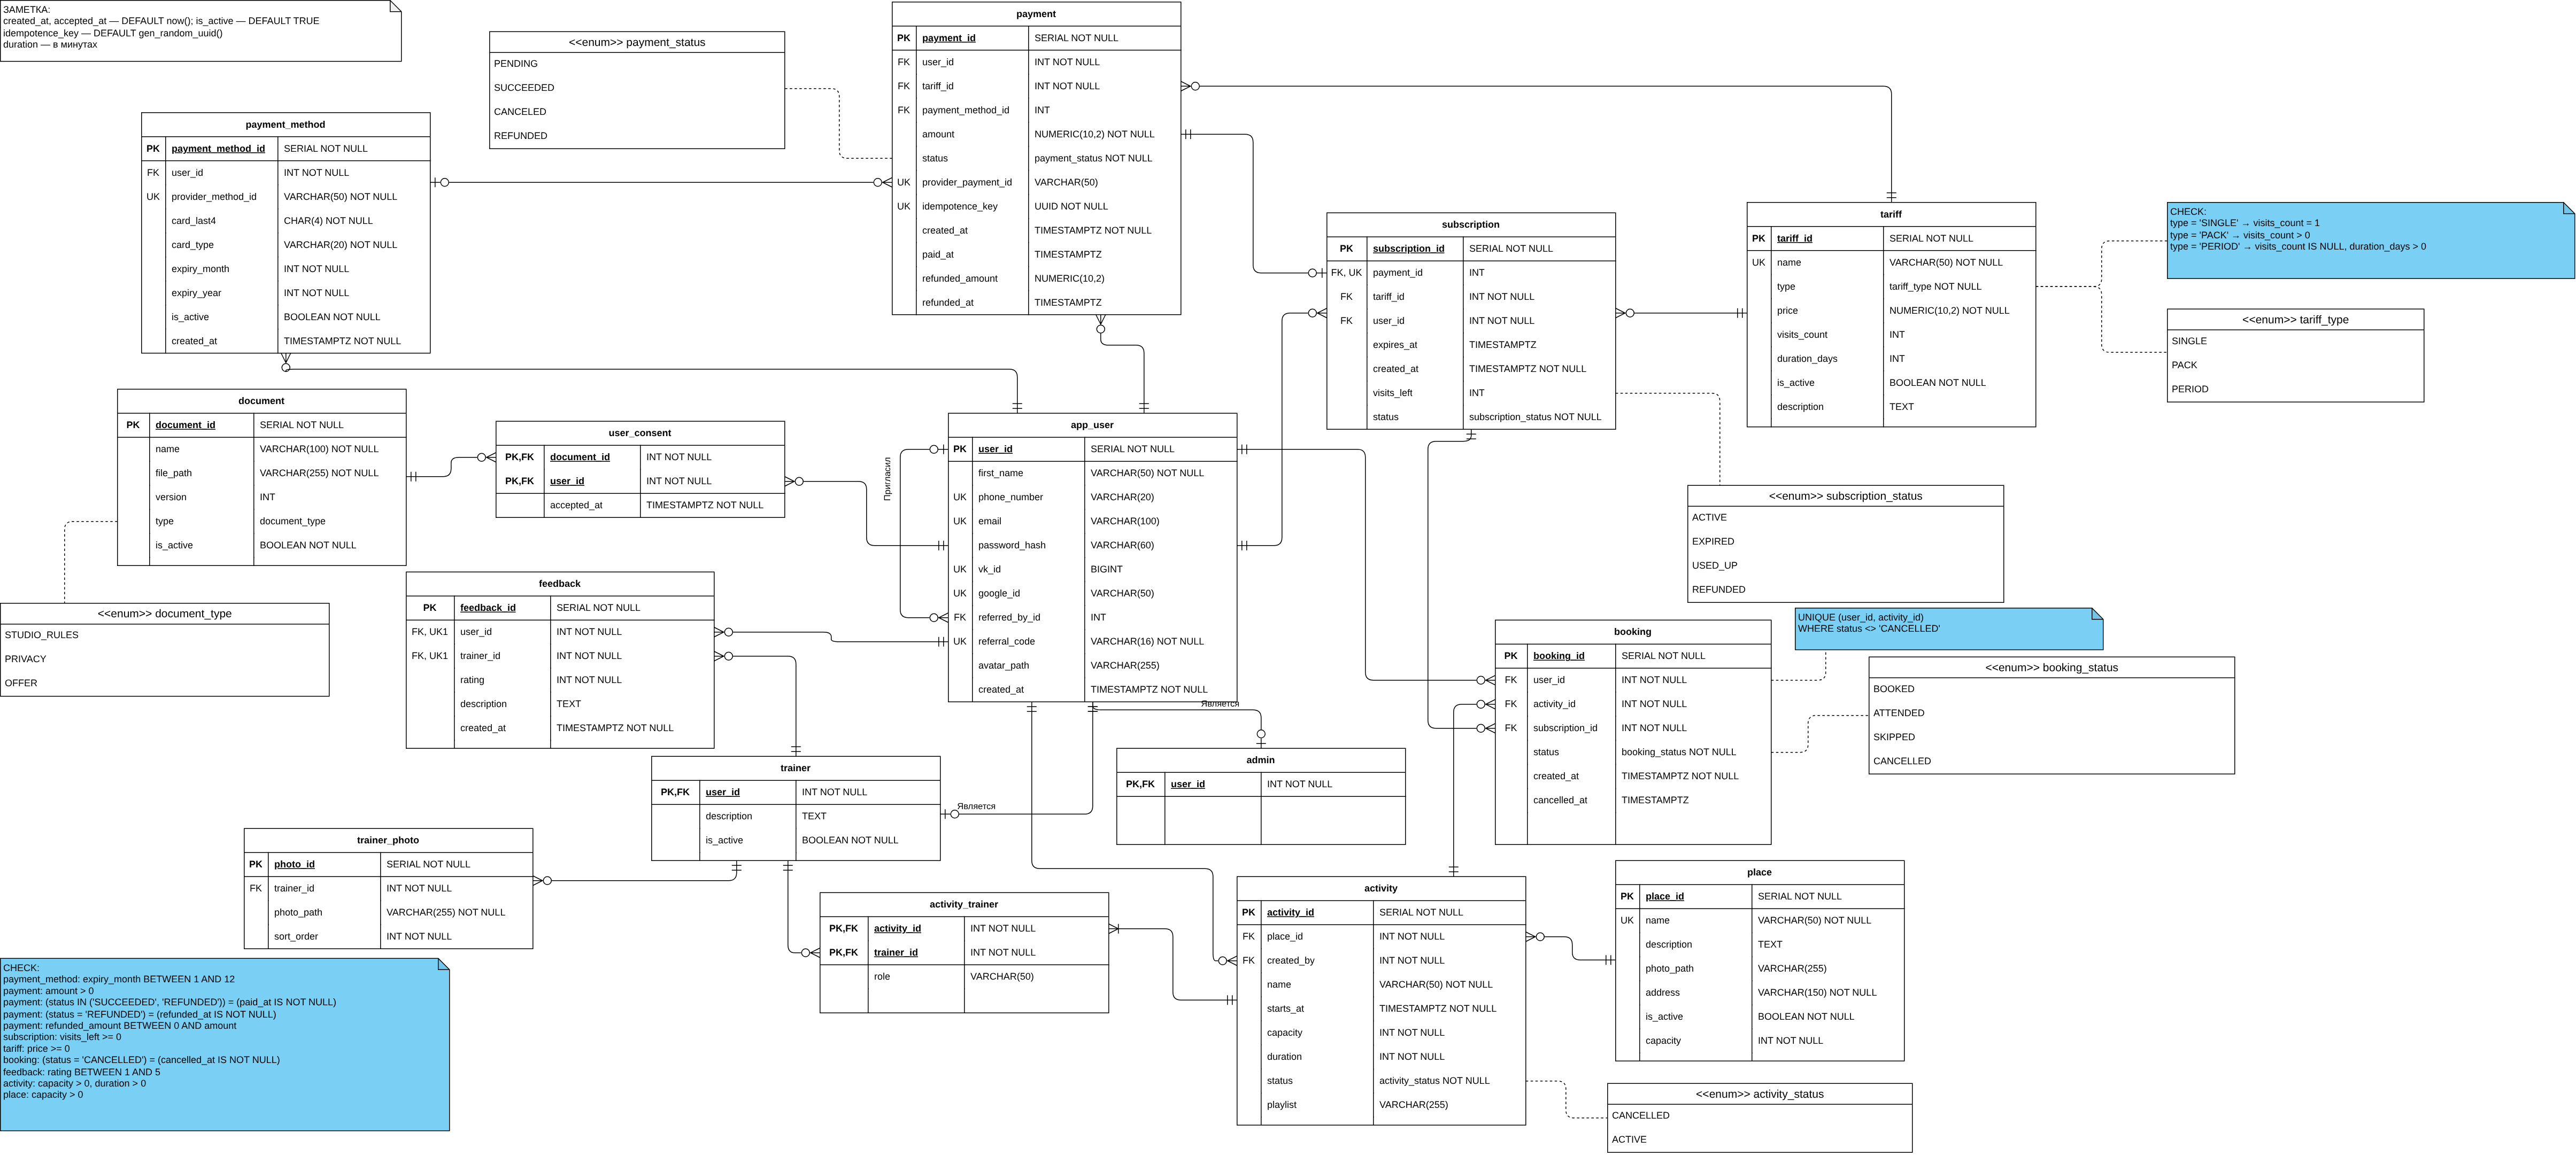
\includegraphics[width=\linewidth,height=0.9\textheight,keepaspectratio]{diagrams/datalogical-model.png}}{\includegraphics[width=\linewidth,height=0.9\textheight,keepaspectratio]{datalogical-model.png}}
  \caption{Даталогическая модель}
  \label{fig:dl}
\end{figure}
\end{landscape}

\end{document}
